\documentclass[../ManualeSviluppatore.tex]{subfiles}

\begin{document}
\section{Strumenti di sviluppo}
	
	Per la generazione del progetto sono necessari i kit di sviluppo Andrid SDK e Java JDK installate nel proprio computer, inoltre la generazione dell'applicativo con risoluzione delle dipendenze è automatica grazie all'uso di Gradle.
	Di seguito si indicano le versioni dei kit di sviluppo utilizzate nel progetto e la descrizione del file gradle e le istruzioni di come eseguirlo nell'ambiente di sviluppo Android Studio.

	\subsection{Android SDK}
		Framework di sviluppo per applicazioni Android.
		\begin{itemize} 
			\item Veesione SDK 24.4.1;
			\item Versione build tools 23.0.3;
			\item Versione target SDK 23;
			\item Versione minima SDK 19.
		\end{itemize}
		
	\subsection{Java JDK}
		Insieme di strumenti di sviluppo per applicazioni Java. 
		\begin{itemize} 
			\item Versione oraclejdk8.
		\end{itemize}
		
	\newpage
	\subsection{Gradle}
	\label{subsec:Gradle}
		Sistema open source per l'automazione dello sviluppo basato su Groovy.
		\begin{itemize} 
			\item Vesione 2.1.0.
		\end{itemize}
		
		\subsubsection{Configurazione gradle Android Studio}
			Per assicurarsi che la \textbf{build} di Gradle funzioni correttamente: in Android Studio cliccare \textbf{File} $\rightarrow$ \textbf{Settings} oppure premere \textbf{CTRL+ALT+S}:
			
		\begin{figure} [h]
			\centering
			\includegraphics[width=\textwidth]{img/settings}
			\label{fig:Settings}
			\caption{Aprire le impostazioni Android Studio}
		\end{figure}
		
		\paragraph*{}
			Nella nuova finestra aperta spostarsi su \textbf{Build, Execution, Deployment} $\rightarrow$ \textbf{Build Tools} $\rightarrow$ \textbf{Gradle}. Spuntare l'opzione \textbf{Use default gradle wrapper (raccommended)} come in figura \ref{fig:SetGradle}:
			
			\begin{figure} [h]
				\centering
				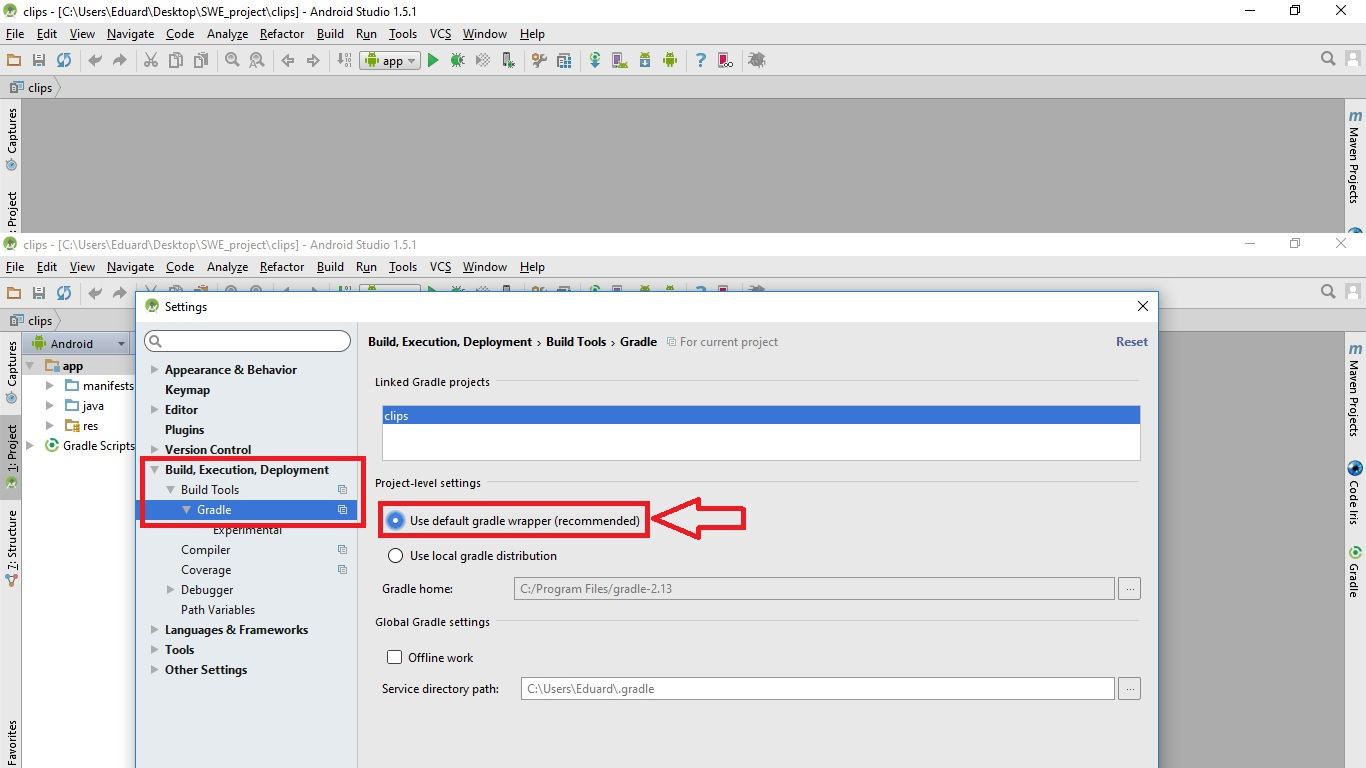
\includegraphics[width=\textwidth]{img/SetGradle}
				\caption{Impostare Gradle correttamente}
				\label{fig:SetGradle}
			\end{figure}
		
		
		\newpage		
		\subsubsection{Contenuto file gradle}
		Nel file gradle vengono dichiarate tutte le dipendenze da risolvere per poter testare, compilare ed eseguire l'applicazione. Di seguito sono riportate le dipendenze dichiarate per l'applicativo. 
		\begin{itemize}
			\item Dichiarazione dei plugin utilizzati
			\lstset{language=Java}
			\begin{lstlisting}
apply plugin: 'com.android.application'
apply plugin: 'com.neenbedankt.android-apt'
			\end{lstlisting}
			\item Dichiarazione dipendenze per gli script di build
			\lstset{language=Java}
			\begin{lstlisting}
buildscript {
    repositories {
        jcenter()
    }
    dependencies {
        classpath 'com.android.tools.build:gradle:2.1.0'
    }
}
			\end{lstlisting}
			\item Dichiarazione della configurazione di Android utilizzata
			\lstset{language=Java}
			\begin{lstlisting}
android {
    compileSdkVersion 23
    buildToolsVersion '23.0.3'

    defaultConfig {
        applicationId "com.leaf.clips"
        minSdkVersion 19
        targetSdkVersion 23
        versionCode 1
        versionName "1.0"
    }
    buildTypes {
        release {
            minifyEnabled true
            shrinkResources true
            proguardFiles getDefaultProguardFile
            	('proguard-android.txt'), 'proguard-rules.pro'
        }
    }
    defaultConfig {
        testInstrumentationRunner "android.support.test.
        	runner.AndroidJUnitRunner"
    }
}

			\end{lstlisting}
			\item Dichiarazione delle dipendenze verso pacchetti esterni utilizzati
				\begin{itemize}
					\item Dipendenze da componenti Android		
						\lstset{language=Java}
						\begin{lstlisting}
compile 'com.android.support:appcompat-v7:23.3.0'
androidTestCompile 'com.android.support:
	appcompat-v7:23.3.0'
androidTestCompile 'com.android.support:
	support-annotations:23.3.0'

compile 'com.android.support:design:23.3.0'
androidTestCompile 'com.android.support:design:23.3.0'
compile 'com.android.support:support-v4:23.3.0'
androidTestCompile 'com.android.support:support-v4:23.3.0'
						\end{lstlisting}
					\item Dipendenze verso Dagger
						\lstset{language=Java}
						\begin{lstlisting}
compile 'com.google.dagger:dagger:2.0'
provided 'com.google.dagger:dagger-compiler:2.0'
provided 'org.glassfish:javax.annotation:10.0-b28'
						\end{lstlisting}
					\item Dipendenze verso JGraphT
						\lstset{language=Java}
						\begin{lstlisting}
compile 'org.jgrapht:jgrapht-core:0.9.1'
						\end{lstlisting}
					\item Dipendenze verso Gson
						\lstset{language=Java}
						\begin{lstlisting}
compile 'com.google.code.gson:gson:2.6.2'
						\end{lstlisting}
					\item Dipendenze verso JUnit(test)
						\lstset{language=Java}
						\begin{lstlisting}
testCompile 'junit:junit:4.12'
androidTestCompile 'com.android.support:
	support-annotations:23.1.1'
androidTestCompile 'com.android.support.test:rules:0.5'
androidTestCompile 'com.android.support.test:runner:0.5'
						\end{lstlisting}
					\item Dipendenze verso Mockito(test)
						\lstset{language=Java}
						\begin{lstlisting}
testCompile 'org.mockito:mockito-core:1.10.19'
						\end{lstlisting}
					\item Dipendenze verso Espresso(test)
						\lstset{language=Java}
						\begin{lstlisting}
androidTestCompile 'com.android.support.test.espresso:
	espresso-core:2.2.2'
androidTestCompile 'com.android.support.test.espresso:
	espresso-web:2.2.2'
androidTestCompile ('com.android.support.test.espresso:
	espresso-contrib:2.2.2') {
    exclude group: 'com.android.support', 
    	module: 'appcompat'
    exclude group: 'com.android.support', 
    	module: 'support-v4'
    exclude module: 'recyclerview-v7'
}
androidTestCompile 'com.android.support.test.espresso:
	espresso-idling-resource:2.2.2'
						\end{lstlisting}
					\item Dipendenze verso FindBugs(analisi statica)
						\lstset{language=Java}
						\begin{lstlisting}
compile 'com.google.code.findbugs:jsr305:2.0.1'
						\end{lstlisting}

				\end{itemize}
		\end{itemize}
\end{document}